\documentclass{article}

% Packages forked from the original template
\usepackage{fancyhdr}
\usepackage{extramarks}
\usepackage{amsmath}
\usepackage{amsthm}
\usepackage{amsfonts}
\usepackage{tikz}
\usepackage[plain]{algorithm}
\usepackage{algpseudocode}

% Extra packages
\usepackage{changepage} % adjustwidth environment
\usepackage{hyperref} % href
\usepackage{xcolor} % colored text
\usepackage{pgfplots}
\usepackage{enumitem} % enumerate with letters
\pgfplotsset{compat=1.18}

\usetikzlibrary{automata,positioning}

% Additional commands
\def\eg{\emph{e.g., }}
\def\ie{\emph{i.e., }}
\def\cf{\emph{c.f., }}
\def\etc{\emph{etc. }}
\def\wrt{\emph{w.r.t. }}
\def\etal{\emph{et al. }}

%
% Basic Document Settings
%

\topmargin=-0.45in
\evensidemargin=0in
\oddsidemargin=0in
\textwidth=6.5in
\textheight=9.0in
\headsep=0.25in

\linespread{1.1}

\pagestyle{fancy}
\lhead{\hmwkClass: \hmwkTitle}
\rhead{\firstxmark}
\lfoot{\lastxmark}
\cfoot{\thepage}

\renewcommand\headrulewidth{0.4pt}
\renewcommand\footrulewidth{0.4pt}

\setlength\parindent{0pt}

%
% Create Problem Sections
%

\newcommand{\enterProblemHeader}[1]{
    \nobreak\extramarks{}{Exercise \arabic{#1} continued on next page\ldots}\nobreak{}
    \nobreak\extramarks{Exercise \arabic{#1} (continued)}{Exercise \arabic{#1} continued on next page\ldots}\nobreak{}
}

\newcommand{\exitProblemHeader}[1]{
    \nobreak\extramarks{Exercise \arabic{#1} (continued)}{Exercise \arabic{#1} continued on next page\ldots}\nobreak{}
    \stepcounter{#1}
    \nobreak\extramarks{Exercise \arabic{#1}}{}\nobreak{}
}

\setcounter{secnumdepth}{0}
\newcounter{partCounter}
\newcounter{homeworkProblemCounter}
\setcounter{homeworkProblemCounter}{1}
\nobreak\extramarks{Exercise \arabic{homeworkProblemCounter}}{}\nobreak{}

%
% Homework Problem Environment
%
% This environment takes an optional argument. When given, it will adjust the
% problem counter. This is useful for when the problems given for your
% assignment aren't sequential. See the last 3 problems of this template for an
% example.
%
\newenvironment{homeworkProblem}[1][-1]{
    \ifnum#1>0
        \setcounter{homeworkProblemCounter}{#1}
    \fi
    \section{Exercise \arabic{homeworkProblemCounter}}
    \setcounter{partCounter}{1}
    \enterProblemHeader{homeworkProblemCounter}
}{
    \exitProblemHeader{homeworkProblemCounter}
}

%
% Homework Details
%   - Title
%   - Due date
%   - Class
%   - Section/Time
%   - Instructor
%   - Author
%

\newcommand{\hmwkTitle}{Assignment 8}
\newcommand{\hmwkDueDate}{June 18, 2024}
\newcommand{\hmwkClass}{Continuous Optimization}
\newcommand{\hmwkAuthorName}{ \textbf{Honglu Ma} \and \textbf{Hiroyasu Akada} \and \textbf{Mathivathana Ayyappan}}

%
% Title Page
%

\title{
    \vspace{2in}
    \textmd{\textbf{\hmwkClass:\ \hmwkTitle}}\\
    \normalsize\vspace{0.1in}\small{Due\ on\ \hmwkDueDate}\\
    \vspace{3in}
}

\author{\hmwkAuthorName}
\date{}

\renewcommand{\part}[1]{\textbf{\large Part \Alph{partCounter}}\stepcounter{partCounter}\\}

%
% Various Helper Commands
%

% Useful for algorithms
\newcommand{\alg}[1]{\textsc{\bfseries \footnotesize #1}}

% For derivatives
\newcommand{\deriv}[1]{\frac{\mathrm{d}}{\mathrm{d}x} (#1)}

% For partial derivatives
\newcommand{\pderiv}[2]{\frac{\partial}{\partial #1} (#2)}

% Integral dx
\newcommand{\dx}{\mathrm{d}x}

% Alias for the Solution section header
\newcommand{\solution}{\textbf{\large Solution}}

% Probability commands: Expectation, Variance, Covariance, Bias
\newcommand{\E}{\mathrm{E}}
\newcommand{\Var}{\mathrm{Var}}
\newcommand{\Cov}{\mathrm{Cov}}
\newcommand{\Bias}{\mathrm{Bias}}

% Norm
\newcommand{\norm}[1]{\left\lVert#1\right\rVert}

% Margined Homework Subsection
\newenvironment{homeworkSubsection}[1]{%
    \subsection*{#1}%
    \begin{adjustwidth}{2.5em}{0pt}%
}{%
    \end{adjustwidth}%
}

\begin{document}

\maketitle

\pagebreak

\begin{homeworkProblem}[1]
    The constraint set $C$ is defined as
    \[
        C := \left\{\begin{pmatrix}
            x_1 \\ x_2
        \end{pmatrix} \in \mathbb{R}^2 \;\Big|\; x_1,\,x_2 \geq 0,\; x_1x_2 = 0 \right\}
    \]
    which are the points lie on the axes of the first quadrant shown in Figure \ref{fig:constraintset1}.
    \begin{figure}[ht]
        \centering
        \begin{tikzpicture}
            % Draw the axes
            \draw[->] (-2,0) -- (3.5,0) node[right] {$x$};
            \draw[->] (0,-2) -- (0,3.5) node[above] {$y$};
        
            % Highlight the entire positive axes in the first quadrant
            \draw[very thick, red] (0,0) -- (3.45,0);
            \draw[very thick, red] (0,0) -- (0,3.45);
        
            % Add tick marks and labels
            \foreach \x in {-1, 1, 2}
                \draw (\x,2pt) -- (\x,-2pt) node[below] {$\x$};
            \foreach \y in {-1, 1, 2}
                \draw (2pt,\y) -- (-2pt,\y) node[left] {$\y$};
        
            % Add a red dot at the origin
            \filldraw[red] (0,0) circle (2pt);
        \end{tikzpicture}
        \caption{Illustration of the constraint set $C$ marked in red.}
        \label{fig:constraintset1}
    \end{figure}

    \begin{homeworkSubsection}{Tangent Cone}
        The tangent cone of a set $C$ at a point $\bar{x} \in C$ is the closure of the set of all feasible directions of $C$ at $\bar{x}$.
        Apparently, the vectors on the axes pointing at positive directions are the feasible directions of $C$ at $\bar{x}$
        and also the closure of such set is itself.

        Thus, the tangent cone to $C$ at $\bar{x} = \begin{pmatrix} 0 \\ 0 \end{pmatrix}$ is
        \[
            T_C(\bar{x}) = \left\{\begin{pmatrix}
                t_1 \\ t_2
            \end{pmatrix} \in \mathbb{R}^2 \;\Big|\; t_1,\,t_2 \geq 0,\; t_1t_2 = 0 
            \right\}
        \]
        as shown in Figure \ref{fig:tangentcone1}.
        \begin{figure}[ht]
            \centering
            \begin{tikzpicture}
                % Draw the axes
                \draw[->] (-2,0) -- (3.5,0) node[right] {$x$};
                \draw[->] (0,-2) -- (0,3.5) node[above] {$y$};
            
                % Highlight the entire positive axes in the first quadrant
                \draw[very thick, red] (0,0) -- (3.45,0);
                \draw[very thick, red] (0,0) -- (0,3.45);
            
                % Add tick marks and labels
                \foreach \x in {-1, 1, 2}
                    \draw (\x,2pt) -- (\x,-2pt) node[below] {$\x$};
                \foreach \y in {-1, 1, 2}
                    \draw (2pt,\y) -- (-2pt,\y) node[left] {$\y$};
            
                % Add a red dot at the origin
                \filldraw[red] (0,0) circle (2pt);
            \end{tikzpicture}
            \caption{Illustration of the tangent cone of $C$ at $\bar{x}$ marked in red.}
            \label{fig:tangentcone1}
        \end{figure}
    \end{homeworkSubsection}
    \begin{homeworkSubsection}{Normal Cone}
        The normal cone of a set $C$ at a point $\bar{x} \in C$ 
        is the set of all vectors $v$ s.t. $\langle v, x-\bar{x}\rangle \leq 0,\,\forall x \in C$.
        Another way to visualize this is that $v$ must form acute angles between all feasible directions of $C$ at $\bar{x}$.
        
        Apparently, the normal cone to $C$ at $\bar{x} = \begin{pmatrix} 0 \\ 0 \end{pmatrix}$ is
        \[
            N_C(\bar{x}) = \left\{\begin{pmatrix}
                n_1 \\ n_2
            \end{pmatrix} \in \mathbb{R}^2 \;\Big|\; n_1,\,n_2 \leq 0
            \right\}
        \]
        as shown in Figure \ref{fig:normalcone1}.
        \begin{figure}[ht]
            \centering
            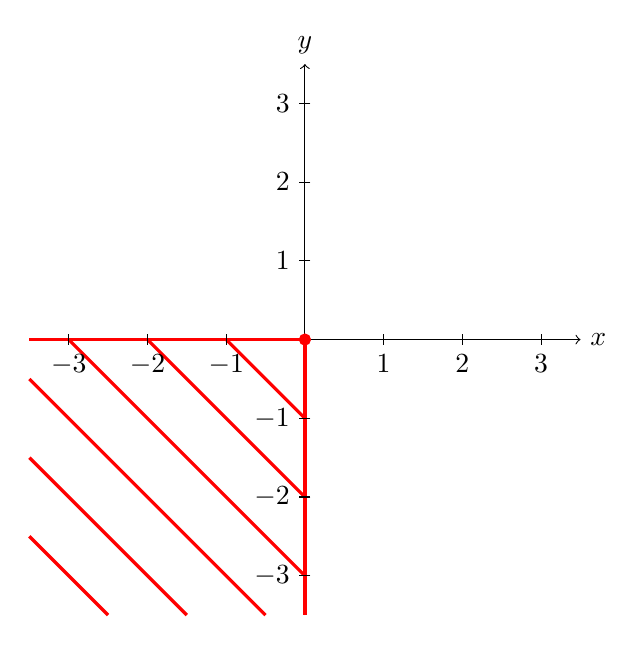
\begin{tikzpicture}
                % Draw the axes
                \draw[->] (-3.5,0) -- (3.5,0) node[right] {$x$};
                \draw[->] (0,-3.5) -- (0,3.5) node[above] {$y$};
    
                % Add a red dot at the origin
                \filldraw[red] (0,0) circle (2pt);
        
                % Highlight the entire positive axes in the first quadrant
                \draw[very thick, red] (0,0) -- (-3.5,0);
                \draw[very thick, red] (0,0) -- (0,-3.5);    
        
                % Dashed lines at 45-degree angles in the third quadrant
                \draw[red, very thick] (-3.5,-2.5) -- (-2.5,-3.5);
                \draw[red, very thick] (-3.5,-1.5) -- (-1.5,-3.5);
                \draw[red, very thick] (-3.5,-0.5) -- (-0.5,-3.5);
                \draw[red, very thick] (-3,0) -- (0,-3);
                \draw[red, very thick] (-2,0) -- (0,-2);
                \draw[red, very thick] (-1,0) -- (0,-1);
                
            
                % Add tick marks and labels
                \foreach \x in {-3, -2, -1, 1, 2, 3}
                    \draw (\x,2pt) -- (\x,-2pt) node[below] {$\x$};
                \foreach \y in {-3, -2, -1, 1, 2, 3}
                    \draw (2pt,\y) -- (-2pt,\y) node[left] {$\y$};
            \end{tikzpicture}
            \caption{Illustration of the normal cone of $C$ at $\bar{x}$ marked in red.}
            \label{fig:normalcone1}    
        \end{figure}
    \end{homeworkSubsection}
\end{homeworkProblem}
\begin{homeworkProblem}[2]
    The constraint set $C$ is defined as
    \[
        C := \left\{\begin{pmatrix}
            x_1 \\ x_2
        \end{pmatrix} \in \mathbb{R}^2 \;\Big|\; |x_1| + |x_2| \leq 1 \right\}
    \]
    as shown in Figure \ref{fig:constraintset2}.
    \begin{figure}
        \centering
        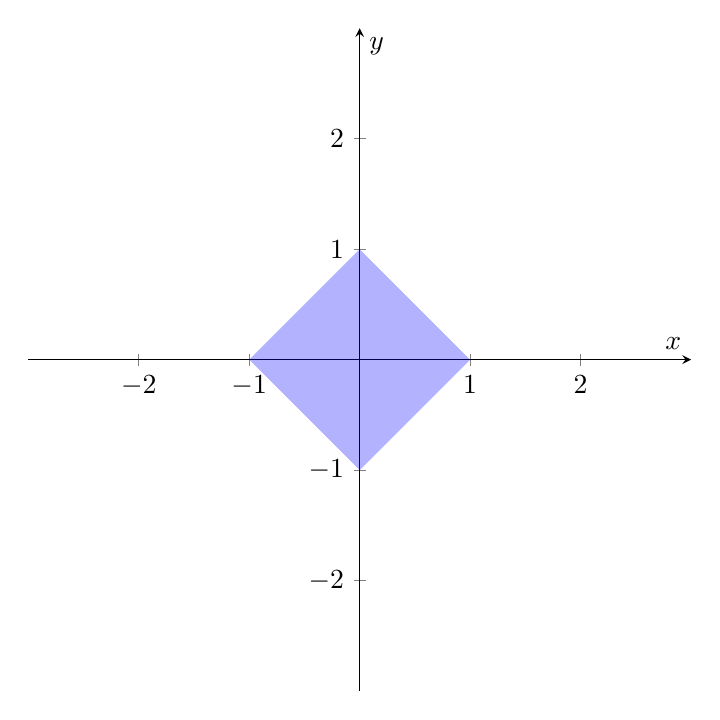
\begin{tikzpicture}
            % Define the axis
            \begin{axis}[
                axis lines = middle,
                xmin = -3, xmax = 3,
                ymin = -3, ymax = 3,
                xlabel = $x$,
                ylabel = $y$,
                xtick = {-2,-1,0,1,2},
                ytick = {-2,-1,0,1,2},
                width=10cm, % Adjust the width of the plot
                height=10cm  % Adjust the height of the plot
            ]
            
            % Draw the square
            \addplot [
                draw=none,
                fill=blue,
                fill opacity=0.3
            ] coordinates { (0,1) (1,0) (0,-1) (-1,0) (0,1) } \closedcycle;
        
            \end{axis}
        \end{tikzpicture}
        \caption{Illustration of the constraint set $C$ as the area covered in blue.}
        \label{fig:constraintset2}    
    \end{figure}
    There are three cases of where the point $\bar{x}$ can land in $C$: 
    \begin{enumerate}[label=\roman*.]
        \item $\bar{x}$ is in the interior of $C$
        \item $\bar{x}$ is on the edges of $C$
        \item $\bar{x}$ is on the vertices $C$
    \end{enumerate}
    \begin{homeworkSubsection}{(i) $\bar{x}$ is in the interior of $C$}
        As shown in Figure \ref{fig:ex2interior}, $\bar{x}$ is in the interior of set $C$.
        Every vector pointing out of $\bar{x}$ in any direction is a feasible direction of $C$ at $\bar{x}$.
        Thus, the tangent cone of $C$ at $\bar{x}$ is the entire $\mathbb{R}^2$
        and the normal cone of $C$ at $\bar{x}$ is $\{0\}$.
        \begin{figure}
            \centering
            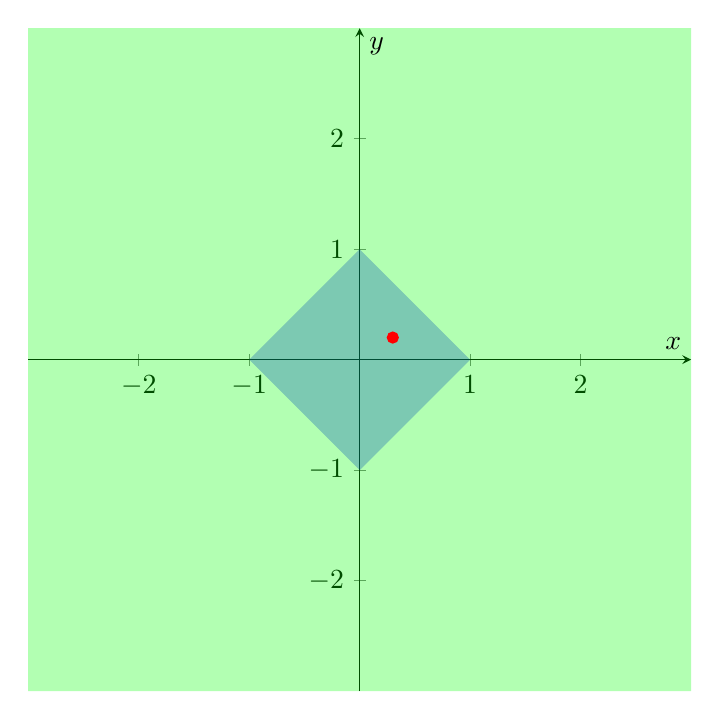
\begin{tikzpicture}
                % Define the axis
                \begin{axis}[
                    axis lines = middle,
                    xmin = -3, xmax = 3,
                    ymin = -3, ymax = 3,
                    xlabel = $x$,
                    ylabel = $y$,
                    xtick = {-2,-1,0,1,2},
                    ytick = {-2,-1,0,1,2},
                    width=10cm, % Adjust the width of the plot
                    height=10cm  % Adjust the height of the plot
                ]
                
                % Draw the square of C
                \addplot [
                    draw=none,
                    fill=blue,
                    fill opacity=0.3
                ] coordinates { (0,1) (1,0) (0,-1) (-1,0) (0,1) } \closedcycle;

                % Draw the area of tangent cone
                \addplot [
                    draw=none,
                    fill=green,
                    fill opacity=0.3
                ] coordinates {(-3, 3) (-3, -3) (3, -3) (3, 3) (-3, 3) } \closedcycle;

                % Plot a single point inside the square
                \addplot[
                    only marks,
                    mark=*,
                    mark size=2pt,
                    color=red
                ] coordinates {(0.3, 0.2)};
                \end{axis}
            \end{tikzpicture}
            \caption{Illustration of $\bar{x}$ in the interior of $C$ marked in red, the tangent cone in green which is the entire $\mathbb{R}^2$.}
            \label{fig:ex2interior}    
        \end{figure}
    \end{homeworkSubsection}
    \begin{homeworkSubsection}{(ii) $\bar{x}$ is on the edges of $C$}
        As shown in Figure \ref{fig:ex2edges}, $\bar{x}$ is on the edges of set $C$.
        The feasible directions of $C$ at $\bar{x}$ are the vectors pointing into $C$.
        Thus, the tangent cone of $C$ at $\bar{x}$ is the area under the line of the edge where $\bar{x}$ lies.
        In case of Figure \ref{fig:ex2edges},
        \[
            T_C(\bar{x}) = \left\{\begin{pmatrix}
                t_1 \\ t_2
            \end{pmatrix} \in \mathbb{R}^2 \;\Big|\; t_1 + t_2 \leq 1 
            \right\}
        \]
        The normal cone of $C$ at $\bar{x}$ is the ray starts from $\bar{x}$ and points out of $C$ and is perpendicular to the edge
        In our case, it can be expressed as 
        \[
            N_C(\bar{x}) = \left\{
                \begin{pmatrix}
                    \frac{1}{2} \\ \frac{1}{2}
                \end{pmatrix} + n\begin{pmatrix}
                \frac{1}{\sqrt{2}} \\ \frac{1}{\sqrt{2}}
            \end{pmatrix} \;\Big|\; n \in \mathbb{R}^2,\,n \geq 0
            \right\}
        \]
        \begin{figure}
            \centering
            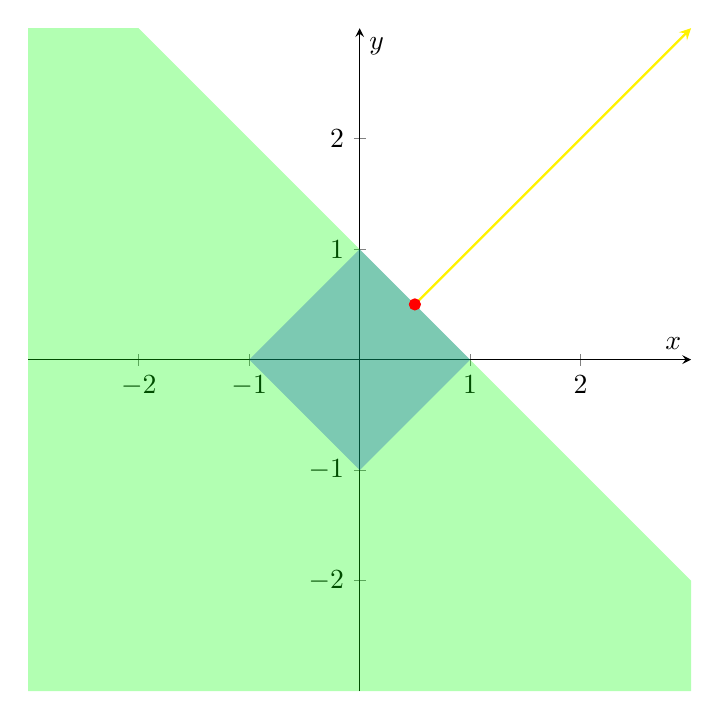
\begin{tikzpicture}
                % Define the axis
                \begin{axis}[
                    axis lines = middle,
                    xmin = -3, xmax = 3,
                    ymin = -3, ymax = 3,
                    xlabel = $x$,
                    ylabel = $y$,
                    xtick = {-2,-1,0,1,2},
                    ytick = {-2,-1,0,1,2},
                    width=10cm, % Adjust the width of the plot
                    height=10cm  % Adjust the height of the plot
                ]
                
                % Draw the square of C
                \addplot [
                    draw=none,
                    fill=blue,
                    fill opacity=0.3
                ] coordinates { (0,1) (1,0) (0,-1) (-1,0) (0,1) } \closedcycle;

                % Draw the area of tangent cone
                \addplot [
                    draw=none,
                    fill=green,
                    fill opacity=0.3
                ] coordinates { (-2, 3) (-3,3) (-3,-3) (3,-3) (3,-2) (-2, 3)} \closedcycle;

                % Plot a single point on the edge of the square
                \addplot[
                    only marks,
                    mark=*,
                    mark size=2pt,
                    color=red
                ] coordinates {(0.5, 0.5)};

                % Draw the vector with arrow head from A to B
                \draw[->, thick, yellow, >=stealth] (0.5, 0.5) -- (3, 3);
                \end{axis}
            \end{tikzpicture}
            \caption{Illustration of $\bar{x}$ on the edges of $C$ marked in red, the tangent cone in green, and the normal cone in yellow.}
            \label{fig:ex2edges}    
        \end{figure}
    \end{homeworkSubsection}
    \begin{homeworkSubsection}{(iii) $\bar{x}$ is on the vertices of $C$}
        As shown in Figure \ref{fig:ex2vertices}, $\bar{x}$ is on the vertices of set $C$.
        The feasible directions of $C$ at $\bar{x}$ are the vectors pointing into $C$.
        Thus, the tangent cone of $C$ at $\bar{x}$ is the area under the two lines of the two edges coincides at $\bar{x}$
        In case of Figure \ref{fig:ex2vertices}, 
        \[  
            T_C(\bar{x}) = \left\{\begin{pmatrix}
                t_1 \\ t_2
            \end{pmatrix} \in \mathbb{R}^2 \;\Big|\; t_1 + t_2 \leq 1 \text{ and } t_1 - t_2 \leq 1 
            \right\}
        \]
        and the normal cone of $C$ at $\bar{x}$ is the area above $C$ where the inverse direction of the two edges surrounds.
        as shown in Figure \ref{fig:ex2vertices},
        \begin{figure}
            \centering
            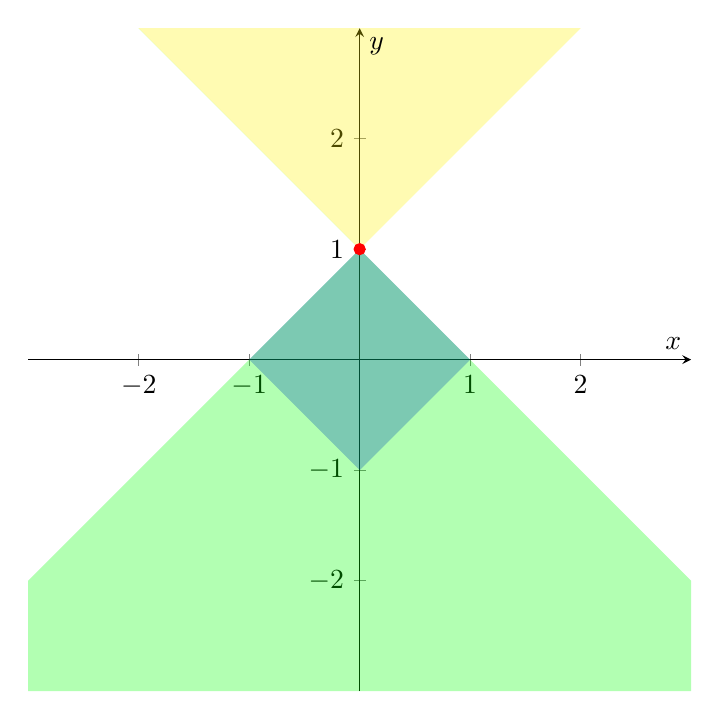
\begin{tikzpicture}
                % Define the axis
                \begin{axis}[
                    axis lines = middle,
                    xmin = -3, xmax = 3,
                    ymin = -3, ymax = 3,
                    xlabel = $x$,
                    ylabel = $y$,
                    xtick = {-2,-1,0,1,2},
                    ytick = {-2,-1,0,1,2},
                    width=10cm, % Adjust the width of the plot
                    height=10cm  % Adjust the height of the plot
                ]
                
                % Draw the square of C
                \addplot [
                    draw=none,
                    fill=blue,
                    fill opacity=0.3
                ] coordinates { (0,1) (1,0) (0,-1) (-1,0) (0,1) } \closedcycle;

                % Draw the area of tangent cone
                \addplot [
                    draw=none,
                    fill=green,
                    fill opacity=0.3
                ] coordinates { (0,1) (-3, -2) (-3,-3) (3,-3) (3,-2) (-2, 3) (0,1)} \closedcycle;

                % Draw the area of normal cone
                \addplot [
                    draw=none,
                    fill=yellow,
                    fill opacity=0.3
                ] coordinates { (0,1) (-2, 3) (2,3) (0,1)} \closedcycle;

                % Plot a single point on the edge of the square
                \addplot[
                    only marks,
                    mark=*,
                    mark size=2pt,
                    color=red
                ] coordinates {(0, 1)};

                \end{axis}
            \end{tikzpicture}
            \caption{Illustration of $\bar{x}$ on the vertices of $C$ marked in red, the tangent cone in green, and the normal cone in yellow.}
            \label{fig:ex2vertices}    
        \end{figure}
        
    \end{homeworkSubsection}
    \end{homeworkProblem}
    \begin{homeworkProblem}[3]
        We are given the set $C$ defined as
        \[
            C = \left\{\begin{pmatrix}
                x_1 \\ x_2
            \end{pmatrix}\in \mathbb{R}^2 \;:\; F(x_1, x_2) \in D\right\}
        \]
        where
        \[
            F(x_1, x_2) = \begin{pmatrix}
                x_1^2 + 3x_2^2 + 2x_2 \\ 3x_1^4 + 2x_2^3 + x_1 + x_2
            \end{pmatrix}
        \]
        and
        \[
            D := \left\{\begin{pmatrix}
                z_1 \\ z_2
            \end{pmatrix} \in \mathbb{R}^2 \;:\;z_1^2 + z_2^2 \leq 1\right\}
        \]
        By Theorem 15.15 (change of coordinates), we know that for a point $\bar{x} \in C$
        and $\bar{z} = F(\bar{x}) \in D$ we can calculate the normal cone of $C$ at $\bar{x}$ as
        \[
            N_C(\bar{x}) = DF(\bar{x})^T N_D(\bar{z})
        \]
        where $DF(\bar{x})$ is the Jacobian matrix of $F$ at $\bar{x}$ and $N_D(\bar{z})$ is the normal cone of $D$ at $\bar{z}$
        and $DF(\bar{x})$ is required to have full rank.

        The Jacobian of $F$ is given by
        \[
            DF(x) = \begin{pmatrix}
                2x_1 & 6x_2 + 2 \\
                12x_1^3 + 1 & 6x_2^2 + 1
            \end{pmatrix}
        \]
        If $\bar{z}$ is in the interior of $D$, then the normal cone of $D$ at $\bar{z}$ is $\{0\}$.
        To be inside of the unit circle, we have $z_1^2 + z_2^2 < 1$.

        If $\bar{z}$ is on the boundary of $D$, then the normal cone of $D$ at $\bar{z}$ is
        \[
            N_D(\bar{z}) = \left\{n\bar{z} \;:\; n \in \mathbb{R}\,,\,n \geq 0\right\}
        \]
        Thus, the normal cone of $C$ at $\bar{x}$ is
        \begin{align*}
            N_C(\bar{x}) &= n\begin{pmatrix}
                2x_1 & 6x_2 + 2 \\
                12x_1^3 + 1 & 6x_2^2 + 1
            \end{pmatrix}^\top \begin{pmatrix}
                x_1^2 + x_2^2 + 2x_2 \\ 3x_1^4 + 2x_2^3 + x_1 + x_2
            \end{pmatrix}\\
            &= n\begin{pmatrix}
                2x_1 & 12x_1^3 + 1 \\
                6x_2 + 2 & 6x_2^2 + 1
            \end{pmatrix} \begin{pmatrix}
                x_1^2 + x_2^2 + 2x_2 \\ 3x_1^4 + 2x_2^3 + x_1 + x_2
            \end{pmatrix}\\
            &= n\begin{pmatrix}
                2x_1(x_1^2 + x_2^2 + 2x_2) + (12x_1^3 + 1)(3x_1^4 + 2x_2^3 + x_1 + x_2)\\
                (6x_2 + 2)(x_1^2 + x_2^2 + 2x_2) + (6x_2^2 + 1)(3x_1^4 + 2x_2^3 + x_1 + x_2)
            \end{pmatrix}\\
            &= n\begin{pmatrix}
                2x_1^3 + 2x_1x_2^2 + 4x_1x_2 + 36x_1^7 + 24x_1^3x_2^3 + 12x_1^4 + 12x_1^3x_2 + 3x_1^4 + 2x_2^3 + x_1 + x_2\\
                (6x_2 + 2)(x_1^2 + x_2^2 + 2x_2) + (6x_2^2 + 1)(3x_1^4 + 2x_2^3 + x_1 + x_2)
            \end{pmatrix}\\
        \end{align*}
    \end{homeworkProblem}
\end{document}
